\documentclass[1p]{elsarticle_modified}
%\bibliographystyle{elsarticle-num}

%\usepackage[colorlinks]{hyperref}
%\usepackage{abbrmath_seonhwa} %\Abb, \Ascr, \Acal ,\Abf, \Afrak
\usepackage{amsfonts}
\usepackage{amssymb}
\usepackage{amsmath}
\usepackage{amsthm}
\usepackage{scalefnt}
\usepackage{amsbsy}
\usepackage{kotex}
\usepackage{caption}
\usepackage{subfig}
\usepackage{color}
\usepackage{graphicx}
\usepackage{xcolor} %% white, black, red, green, blue, cyan, magenta, yellow
\usepackage{float}
\usepackage{setspace}
\usepackage{hyperref}

\usepackage{tikz}
\usetikzlibrary{arrows}

\usepackage{multirow}
\usepackage{array} % fixed length table
\usepackage{hhline}

%%%%%%%%%%%%%%%%%%%%%
\makeatletter
\renewcommand*\env@matrix[1][\arraystretch]{%
	\edef\arraystretch{#1}%
	\hskip -\arraycolsep
	\let\@ifnextchar\new@ifnextchar
	\array{*\c@MaxMatrixCols c}}
\makeatother %https://tex.stackexchange.com/questions/14071/how-can-i-increase-the-line-spacing-in-a-matrix
%%%%%%%%%%%%%%%

\usepackage[normalem]{ulem}

\newcommand{\msout}[1]{\ifmmode\text{\sout{\ensuremath{#1}}}\else\sout{#1}\fi}
%SOURCE: \msout is \stkout macro in https://tex.stackexchange.com/questions/20609/strikeout-in-math-mode

\newcommand{\cancel}[1]{
	\ifmmode
	{\color{red}\msout{#1}}
	\else
	{\color{red}\sout{#1}}
	\fi
}

\newcommand{\add}[1]{
	{\color{blue}\uwave{#1}}
}

\newcommand{\replace}[2]{
	\ifmmode
	{\color{red}\msout{#1}}{\color{blue}\uwave{#2}}
	\else
	{\color{red}\sout{#1}}{\color{blue}\uwave{#2}}
	\fi
}

\newcommand{\Sol}{\mathcal{S}} %segment
\newcommand{\D}{D} %diagram
\newcommand{\A}{\mathcal{A}} %arc


%%%%%%%%%%%%%%%%%%%%%%%%%%%%%5 test

\def\sl{\operatorname{\textup{SL}}(2,\Cbb)}
\def\psl{\operatorname{\textup{PSL}}(2,\Cbb)}
\def\quan{\mkern 1mu \triangleright \mkern 1mu}

\theoremstyle{definition}
\newtheorem{thm}{Theorem}[section]
\newtheorem{prop}[thm]{Proposition}
\newtheorem{lem}[thm]{Lemma}
\newtheorem{ques}[thm]{Question}
\newtheorem{cor}[thm]{Corollary}
\newtheorem{defn}[thm]{Definition}
\newtheorem{exam}[thm]{Example}
\newtheorem{rmk}[thm]{Remark}
\newtheorem{alg}[thm]{Algorithm}

\newcommand{\I}{\sqrt{-1}}
\begin{document}

%\begin{frontmatter}
%
%\title{Boundary parabolic representations of knots up to 8 crossings}
%
%%% Group authors per affiliation:
%\author{Yunhi Cho} 
%\address{Department of Mathematics, University of Seoul, Seoul, Korea}
%\ead{yhcho@uos.ac.kr}
%
%
%\author{Seonhwa Kim} %\fnref{s_kim}}
%\address{Center for Geometry and Physics, Institute for Basic Science, Pohang, 37673, Korea}
%\ead{ryeona17@ibs.re.kr}
%
%\author{Hyuk Kim}
%\address{Department of Mathematical Sciences, Seoul National University, Seoul 08826, Korea}
%\ead{hyukkim@snu.ac.kr}
%
%\author{Seokbeom Yoon}
%\address{Department of Mathematical Sciences, Seoul National University, Seoul, 08826,  Korea}
%\ead{sbyoon15@snu.ac.kr}
%
%\begin{abstract}
%We find all boundary parabolic representation of knots up to 8 crossings.
%
%\end{abstract}
%\begin{keyword}
%    \MSC[2010] 57M25 
%\end{keyword}
%
%\end{frontmatter}

%\linenumbers
%\tableofcontents
%
\newcommand\colored[1]{\textcolor{white}{\rule[-0.35ex]{0.8em}{1.4ex}}\kern-0.8em\color{red} #1}%
%\newcommand\colored[1]{\textcolor{white}{ #1}\kern-2.17ex	\textcolor{white}{ #1}\kern-1.81ex	\textcolor{white}{ #1}\kern-2.15ex\color{red}#1	}

{\Large $\underline{12a_{0126}~(K12a_{0126})}$}

\setlength{\tabcolsep}{10pt}
\renewcommand{\arraystretch}{1.6}
\vspace{1cm}\begin{tabular}{m{100pt}>{\centering\arraybackslash}m{274pt}}
\multirow{5}{120pt}{
	\centering
	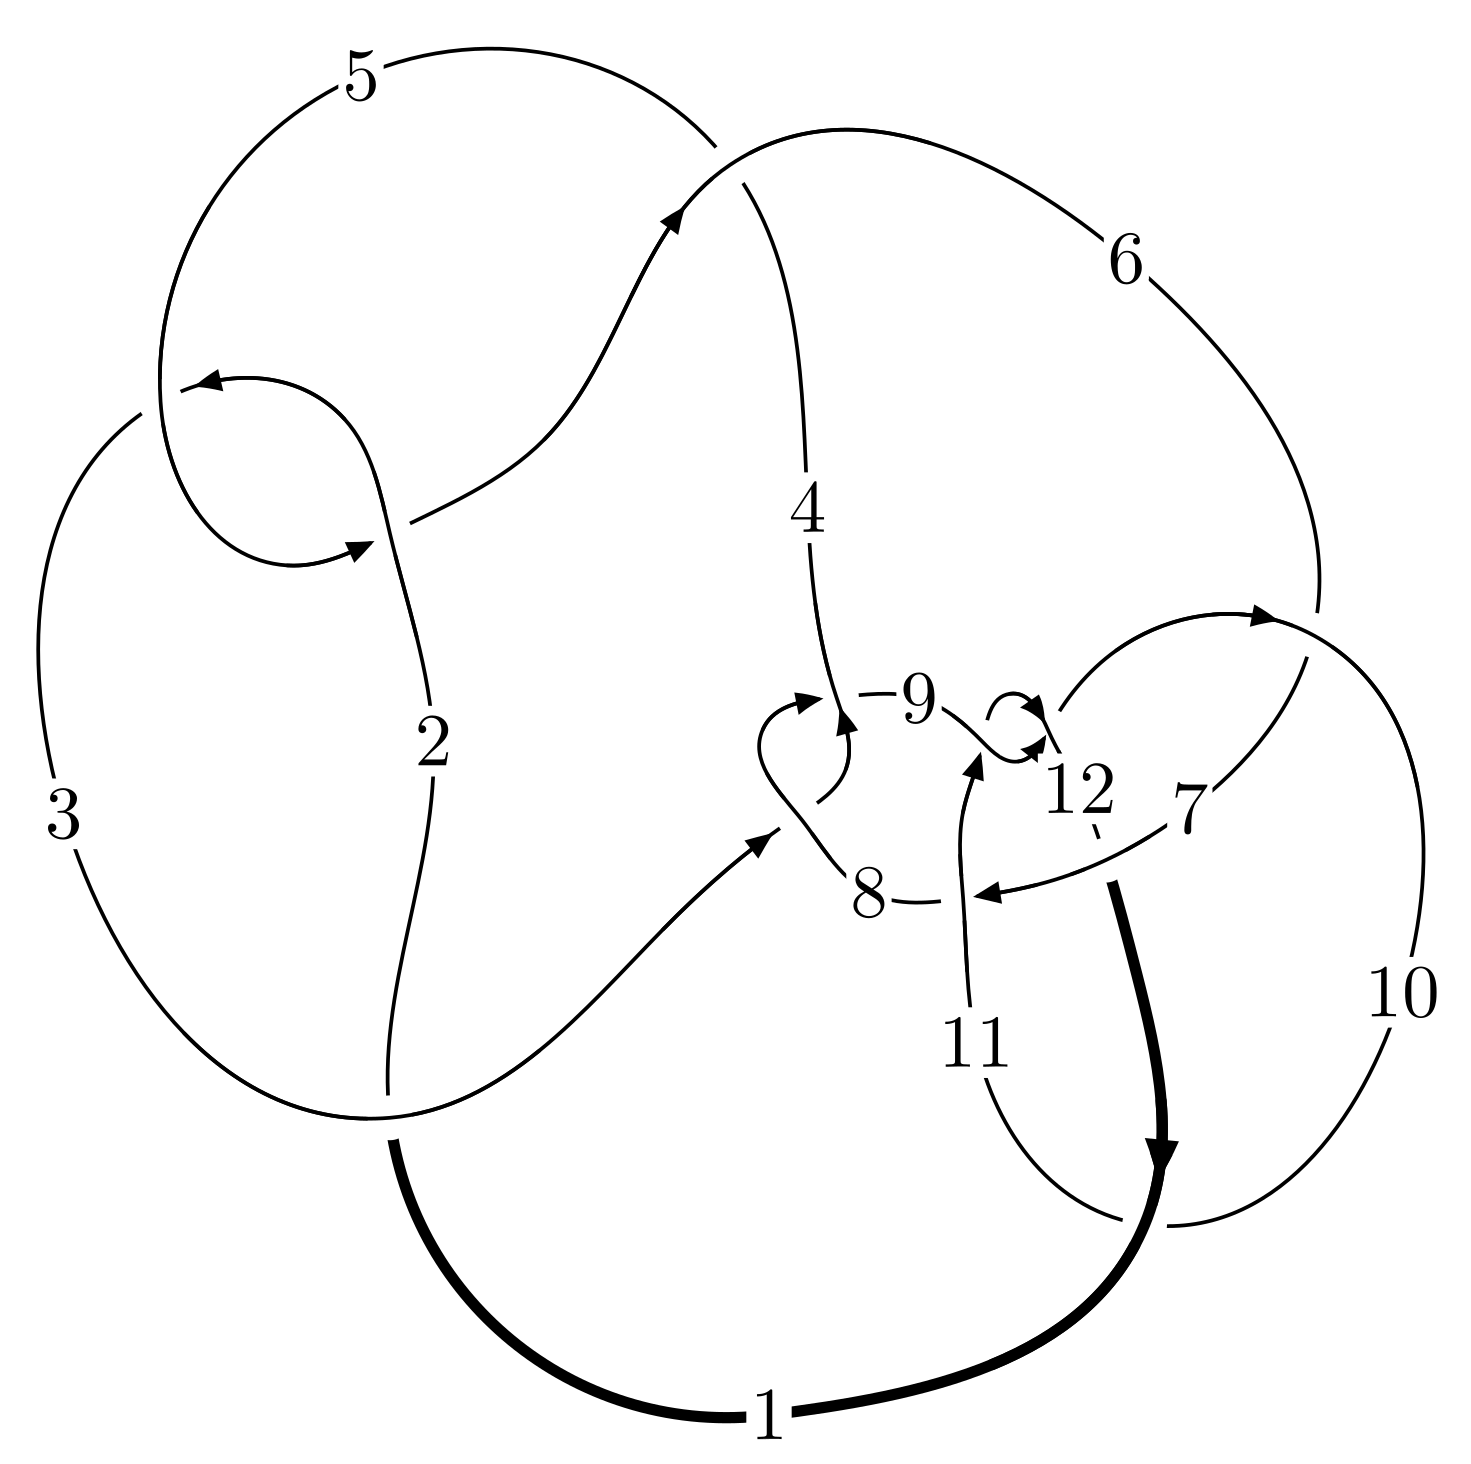
\includegraphics[width=112pt]{../../../GIT/diagram.site/Diagrams/png/927_12a_0126.png}\\
\ \ \ A knot diagram\footnotemark}&
\allowdisplaybreaks
\textbf{Linearized knot diagam} \\
\cline{2-2}
 &
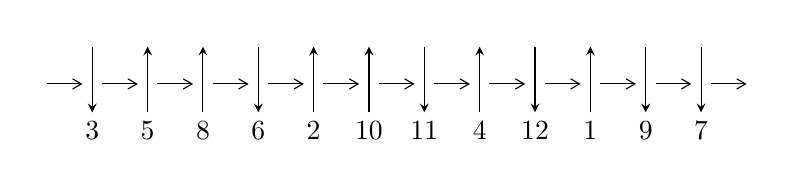
\begin{tikzpicture}[x=20pt, y=17pt]
	% nodes
	\node (C0) at (0, 0) {};
	\node (C1) at (1, 0) {};
	\node (C1U) at (1, +1) {};
	\node (C1D) at (1, -1) {3};

	\node (C2) at (2, 0) {};
	\node (C2U) at (2, +1) {};
	\node (C2D) at (2, -1) {5};

	\node (C3) at (3, 0) {};
	\node (C3U) at (3, +1) {};
	\node (C3D) at (3, -1) {8};

	\node (C4) at (4, 0) {};
	\node (C4U) at (4, +1) {};
	\node (C4D) at (4, -1) {6};

	\node (C5) at (5, 0) {};
	\node (C5U) at (5, +1) {};
	\node (C5D) at (5, -1) {2};

	\node (C6) at (6, 0) {};
	\node (C6U) at (6, +1) {};
	\node (C6D) at (6, -1) {10};

	\node (C7) at (7, 0) {};
	\node (C7U) at (7, +1) {};
	\node (C7D) at (7, -1) {11};

	\node (C8) at (8, 0) {};
	\node (C8U) at (8, +1) {};
	\node (C8D) at (8, -1) {4};

	\node (C9) at (9, 0) {};
	\node (C9U) at (9, +1) {};
	\node (C9D) at (9, -1) {12};

	\node (C10) at (10, 0) {};
	\node (C10U) at (10, +1) {};
	\node (C10D) at (10, -1) {1};

	\node (C11) at (11, 0) {};
	\node (C11U) at (11, +1) {};
	\node (C11D) at (11, -1) {9};

	\node (C12) at (12, 0) {};
	\node (C12U) at (12, +1) {};
	\node (C12D) at (12, -1) {7};
	\node (C13) at (13, 0) {};

	% arrows
	\draw[->,>={angle 60}]
	(C0) edge (C1) (C1) edge (C2) (C2) edge (C3) (C3) edge (C4) (C4) edge (C5) (C5) edge (C6) (C6) edge (C7) (C7) edge (C8) (C8) edge (C9) (C9) edge (C10) (C10) edge (C11) (C11) edge (C12) (C12) edge (C13) ;	\draw[->,>=stealth]
	(C1U) edge (C1D) (C2D) edge (C2U) (C3D) edge (C3U) (C4U) edge (C4D) (C5D) edge (C5U) (C6D) edge (C6U) (C7U) edge (C7D) (C8D) edge (C8U) (C9U) edge (C9D) (C10D) edge (C10U) (C11U) edge (C11D) (C12U) edge (C12D) ;
	\end{tikzpicture} \\
\hhline{~~} \\& 
\textbf{Solving Sequence} \\ \cline{2-2} 
 &
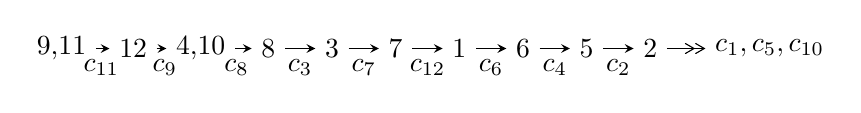
\begin{tikzpicture}[x=23pt, y=7pt]
	% node
	\node (A0) at (-1/8, 0) {9,11};
	\node (A1) at (1, 0) {12};
	\node (A2) at (33/16, 0) {4,10};
	\node (A3) at (25/8, 0) {8};
	\node (A4) at (33/8, 0) {3};
	\node (A5) at (41/8, 0) {7};
	\node (A6) at (49/8, 0) {1};
	\node (A7) at (57/8, 0) {6};
	\node (A8) at (65/8, 0) {5};
	\node (A9) at (73/8, 0) {2};
	\node (C1) at (1/2, -1) {$c_{11}$};
	\node (C2) at (3/2, -1) {$c_{9}$};
	\node (C3) at (21/8, -1) {$c_{8}$};
	\node (C4) at (29/8, -1) {$c_{3}$};
	\node (C5) at (37/8, -1) {$c_{7}$};
	\node (C6) at (45/8, -1) {$c_{12}$};
	\node (C7) at (53/8, -1) {$c_{6}$};
	\node (C8) at (61/8, -1) {$c_{4}$};
	\node (C9) at (69/8, -1) {$c_{2}$};
	\node (A10) at (11, 0) {$c_{1},c_{5},c_{10}$};

	% edge
	\draw[->,>=stealth]	
	(A0) edge (A1) (A1) edge (A2) (A2) edge (A3) (A3) edge (A4) (A4) edge (A5) (A5) edge (A6) (A6) edge (A7) (A7) edge (A8) (A8) edge (A9) ;
	\draw[->>,>={angle 60}]	
	(A9) edge (A10);
\end{tikzpicture} \\ 

\end{tabular} \\

\footnotetext{
The image of knot diagram is generated by the software ``\textbf{Draw programme}" developed by Andrew Bartholomew(\url{http://www.layer8.co.uk/maths/draw/index.htm\#Running-draw}), where we modified some parts for our purpose(\url{https://github.com/CATsTAILs/LinksPainter}).
}\phantom \\ \newline 
\centering \textbf{Ideals for irreducible components\footnotemark of $X_{\text{par}}$} 
 
\begin{align*}
I^u_{1}&=\langle 
-1.19568\times10^{514} u^{123}+1.78570\times10^{514} u^{122}+\cdots+1.37373\times10^{514} b+9.44655\times10^{513},\\
\phantom{I^u_{1}}&\phantom{= \langle  }-8.50500\times10^{513} u^{123}+2.28055\times10^{514} u^{122}+\cdots+6.86865\times10^{513} a+3.75076\times10^{514},\\
\phantom{I^u_{1}}&\phantom{= \langle  }u^{124}-3 u^{123}+\cdots-17 u+1\rangle \\
I^u_{2}&=\langle 
- u^4 b+u^3 b+2 u^4+u^2 b-4 u^3+b^2- b+u+2,\;a,\;u^5- u^4-2 u^3+u^2+u+1\rangle \\
\\
\end{align*}
\raggedright * 2 irreducible components of $\dim_{\mathbb{C}}=0$, with total 134 representations.\\
\footnotetext{All coefficients of polynomials are rational numbers. But the coefficients are sometimes approximated in decimal forms when there is not enough margin.}
\newpage
\renewcommand{\arraystretch}{1}
\centering \section*{I. $I^u_{1}= \langle -1.20\times10^{514} u^{123}+1.79\times10^{514} u^{122}+\cdots+1.37\times10^{514} b+9.45\times10^{513},\;-8.51\times10^{513} u^{123}+2.28\times10^{514} u^{122}+\cdots+6.87\times10^{513} a+3.75\times10^{514},\;u^{124}-3 u^{123}+\cdots-17 u+1 \rangle$}
\flushleft \textbf{(i) Arc colorings}\\
\begin{tabular}{m{7pt} m{180pt} m{7pt} m{180pt} }
\flushright $a_{9}=$&$\begin{pmatrix}0\\u\end{pmatrix}$ \\
\flushright $a_{11}=$&$\begin{pmatrix}1\\0\end{pmatrix}$ \\
\flushright $a_{12}=$&$\begin{pmatrix}1\\u^2\end{pmatrix}$ \\
\flushright $a_{4}=$&$\begin{pmatrix}1.23823 u^{123}-3.32023 u^{122}+\cdots+92.0435 u-5.46069\\0.870390 u^{123}-1.29989 u^{122}+\cdots+18.1293 u-0.687657\end{pmatrix}$ \\
\flushright $a_{10}=$&$\begin{pmatrix}- u\\- u^3+u\end{pmatrix}$ \\
\flushright $a_{8}=$&$\begin{pmatrix}0.636769 u^{123}-3.20862 u^{122}+\cdots+84.3954 u-2.94586\\-1.14946 u^{123}+2.37316 u^{122}+\cdots-41.7539 u+2.55020\end{pmatrix}$ \\
\flushright $a_{3}=$&$\begin{pmatrix}2.25351 u^{123}-8.02311 u^{122}+\cdots+332.546 u-26.9028\\-0.106456 u^{123}+1.24630 u^{122}+\cdots-6.66420 u+1.61535\end{pmatrix}$ \\
\flushright $a_{7}=$&$\begin{pmatrix}-0.512693 u^{123}-0.835457 u^{122}+\cdots+42.6415 u-0.395659\\-1.14946 u^{123}+2.37316 u^{122}+\cdots-41.7539 u+2.55020\end{pmatrix}$ \\
\flushright $a_{1}=$&$\begin{pmatrix}-0.363633 u^{123}+0.445779 u^{122}+\cdots+7.87842 u-3.65412\\0.170523 u^{123}-0.430689 u^{122}+\cdots-0.767532 u+0.281487\end{pmatrix}$ \\
\flushright $a_{6}=$&$\begin{pmatrix}0.626018 u^{123}-2.92628 u^{122}+\cdots+64.5489 u-1.65616\\-1.38877 u^{123}+2.78861 u^{122}+\cdots-42.2698 u+2.48540\end{pmatrix}$ \\
\flushright $a_{5}=$&$\begin{pmatrix}2.64583 u^{123}-8.44868 u^{122}+\cdots+327.721 u-25.5158\\0.318080 u^{123}+0.453649 u^{122}+\cdots+6.76485 u+0.672544\end{pmatrix}$ \\
\flushright $a_{2}=$&$\begin{pmatrix}1.13479 u^{123}-5.07219 u^{122}+\cdots+147.722 u-2.40535\\-0.709729 u^{123}+1.24243 u^{122}+\cdots-53.4260 u+3.18946\end{pmatrix}$\\&\end{tabular}
\flushleft \textbf{(ii) Obstruction class $= -1$}\\~\\
\flushleft \textbf{(iii) Cusp Shapes $= 6.43594 u^{123}-17.2046 u^{122}+\cdots-79.2712 u+10.6191$}\\~\\
\newpage\renewcommand{\arraystretch}{1}
\flushleft \textbf{(iv) u-Polynomials at the component}\newline \\
\begin{tabular}{m{50pt}|m{274pt}}
Crossings & \hspace{64pt}u-Polynomials at each crossing \\
\hline $$\begin{aligned}c_{1},c_{4}\end{aligned}$$&$\begin{aligned}
&u^{124}+42 u^{123}+\cdots+2 u+1
\end{aligned}$\\
\hline $$\begin{aligned}c_{2},c_{5}\end{aligned}$$&$\begin{aligned}
&u^{124}+6 u^{123}+\cdots+2 u+1
\end{aligned}$\\
\hline $$\begin{aligned}c_{3},c_{8}\end{aligned}$$&$\begin{aligned}
&u^{124}- u^{123}+\cdots+5120 u+1024
\end{aligned}$\\
\hline $$\begin{aligned}c_{6}\end{aligned}$$&$\begin{aligned}
&u^{124}-3 u^{123}+\cdots+1975 u+1031
\end{aligned}$\\
\hline $$\begin{aligned}c_{7}\end{aligned}$$&$\begin{aligned}
&u^{124}+3 u^{123}+\cdots-376993 u-48793
\end{aligned}$\\
\hline $$\begin{aligned}c_{9},c_{11}\end{aligned}$$&$\begin{aligned}
&u^{124}-3 u^{123}+\cdots-17 u+1
\end{aligned}$\\
\hline $$\begin{aligned}c_{10}\end{aligned}$$&$\begin{aligned}
&u^{124}+21 u^{123}+\cdots+3 u+1
\end{aligned}$\\
\hline $$\begin{aligned}c_{12}\end{aligned}$$&$\begin{aligned}
&u^{124}-9 u^{123}+\cdots-3 u+1
\end{aligned}$\\
\hline
\end{tabular}\\~\\
\newpage\renewcommand{\arraystretch}{1}
\flushleft \textbf{(v) Riley Polynomials at the component}\newline \\
\begin{tabular}{m{50pt}|m{274pt}}
Crossings & \hspace{64pt}Riley Polynomials at each crossing \\
\hline $$\begin{aligned}c_{1},c_{4}\end{aligned}$$&$\begin{aligned}
&y^{124}+86 y^{123}+\cdots-1250 y+1
\end{aligned}$\\
\hline $$\begin{aligned}c_{2},c_{5}\end{aligned}$$&$\begin{aligned}
&y^{124}+42 y^{123}+\cdots+2 y+1
\end{aligned}$\\
\hline $$\begin{aligned}c_{3},c_{8}\end{aligned}$$&$\begin{aligned}
&y^{124}-55 y^{123}+\cdots-26214400 y+1048576
\end{aligned}$\\
\hline $$\begin{aligned}c_{6}\end{aligned}$$&$\begin{aligned}
&y^{124}+131 y^{123}+\cdots+138554707 y+1062961
\end{aligned}$\\
\hline $$\begin{aligned}c_{7}\end{aligned}$$&$\begin{aligned}
&y^{124}+83 y^{123}+\cdots-318551403169 y+2380756849
\end{aligned}$\\
\hline $$\begin{aligned}c_{9},c_{11}\end{aligned}$$&$\begin{aligned}
&y^{124}-85 y^{123}+\cdots-17 y+1
\end{aligned}$\\
\hline $$\begin{aligned}c_{10}\end{aligned}$$&$\begin{aligned}
&y^{124}+3 y^{123}+\cdots-17 y+1
\end{aligned}$\\
\hline $$\begin{aligned}c_{12}\end{aligned}$$&$\begin{aligned}
&y^{124}-21 y^{123}+\cdots-9 y+1
\end{aligned}$\\
\hline
\end{tabular}\\~\\
\newpage\flushleft \textbf{(vi) Complex Volumes and Cusp Shapes}
$$\begin{array}{c|c|c}  
\text{Solutions to }I^u_{1}& \I (\text{vol} + \sqrt{-1}CS) & \text{Cusp shape}\\
 \hline 
\begin{aligned}
u &= -0.993111 + 0.053773 I \\
a &= \phantom{-}0.304536 - 0.731943 I \\
b &= -3.32424 + 1.95187 I\end{aligned}
 & -1.07695 + 2.69734 I & \phantom{-0.000000 } 0 \\ \hline\begin{aligned}
u &= -0.993111 - 0.053773 I \\
a &= \phantom{-}0.304536 + 0.731943 I \\
b &= -3.32424 - 1.95187 I\end{aligned}
 & -1.07695 - 2.69734 I & \phantom{-0.000000 } 0 \\ \hline\begin{aligned}
u &= \phantom{-}0.102129 + 0.978954 I \\
a &= \phantom{-}0.989365 + 0.390154 I \\
b &= -0.047901 - 0.761141 I\end{aligned}
 & \phantom{-}2.42925 + 1.41500 I & \phantom{-0.000000 } 0 \\ \hline\begin{aligned}
u &= \phantom{-}0.102129 - 0.978954 I \\
a &= \phantom{-}0.989365 - 0.390154 I \\
b &= -0.047901 + 0.761141 I\end{aligned}
 & \phantom{-}2.42925 - 1.41500 I & \phantom{-0.000000 } 0 \\ \hline\begin{aligned}
u &= \phantom{-}0.960892 + 0.127416 I \\
a &= -1.02339 - 1.08127 I \\
b &= \phantom{-}0.001099 + 0.605351 I\end{aligned}
 & -0.61080 - 4.13411 I & \phantom{-0.000000 } 0 \\ \hline\begin{aligned}
u &= \phantom{-}0.960892 - 0.127416 I \\
a &= -1.02339 + 1.08127 I \\
b &= \phantom{-}0.001099 - 0.605351 I\end{aligned}
 & -0.61080 + 4.13411 I & \phantom{-0.000000 } 0 \\ \hline\begin{aligned}
u &= \phantom{-}1.023570 + 0.155026 I \\
a &= -1.305260 + 0.028917 I \\
b &= -1.114000 - 0.105881 I\end{aligned}
 & -2.35592 - 4.60181 I & \phantom{-0.000000 } 0 \\ \hline\begin{aligned}
u &= \phantom{-}1.023570 - 0.155026 I \\
a &= -1.305260 - 0.028917 I \\
b &= -1.114000 + 0.105881 I\end{aligned}
 & -2.35592 + 4.60181 I & \phantom{-0.000000 } 0 \\ \hline\begin{aligned}
u &= \phantom{-}0.103026 + 1.034420 I \\
a &= -0.420200 + 0.976552 I \\
b &= \phantom{-}0.04073 - 1.77407 I\end{aligned}
 & \phantom{-}2.86743 + 4.32090 I & \phantom{-0.000000 } 0 \\ \hline\begin{aligned}
u &= \phantom{-}0.103026 - 1.034420 I \\
a &= -0.420200 - 0.976552 I \\
b &= \phantom{-}0.04073 + 1.77407 I\end{aligned}
 & \phantom{-}2.86743 - 4.32090 I & \phantom{-0.000000 } 0\\
 \hline 
 \end{array}$$\newpage$$\begin{array}{c|c|c}  
\text{Solutions to }I^u_{1}& \I (\text{vol} + \sqrt{-1}CS) & \text{Cusp shape}\\
 \hline 
\begin{aligned}
u &= \phantom{-}0.565867 + 0.885433 I \\
a &= \phantom{-}0.551247 - 1.154640 I \\
b &= -0.07495 + 1.59124 I\end{aligned}
 & \phantom{-}8.29858 - 2.50158 I & \phantom{-0.000000 } 0 \\ \hline\begin{aligned}
u &= \phantom{-}0.565867 - 0.885433 I \\
a &= \phantom{-}0.551247 + 1.154640 I \\
b &= -0.07495 - 1.59124 I\end{aligned}
 & \phantom{-}8.29858 + 2.50158 I & \phantom{-0.000000 } 0 \\ \hline\begin{aligned}
u &= -0.945786 + 0.068110 I \\
a &= -0.833155 - 0.190342 I \\
b &= -1.05192 + 3.40683 I\end{aligned}
 & -0.377994 + 0.348299 I & \phantom{-0.000000 } 0 \\ \hline\begin{aligned}
u &= -0.945786 - 0.068110 I \\
a &= -0.833155 + 0.190342 I \\
b &= -1.05192 - 3.40683 I\end{aligned}
 & -0.377994 - 0.348299 I & \phantom{-0.000000 } 0 \\ \hline\begin{aligned}
u &= -0.272313 + 1.015970 I \\
a &= -0.756103 - 0.410555 I \\
b &= -0.170492 + 0.784563 I\end{aligned}
 & -2.52436 + 2.17800 I & \phantom{-0.000000 } 0 \\ \hline\begin{aligned}
u &= -0.272313 - 1.015970 I \\
a &= -0.756103 + 0.410555 I \\
b &= -0.170492 - 0.784563 I\end{aligned}
 & -2.52436 - 2.17800 I & \phantom{-0.000000 } 0 \\ \hline\begin{aligned}
u &= -1.069430 + 0.043655 I \\
a &= \phantom{-}0.723563 + 0.551297 I \\
b &= -1.14955 - 3.56938 I\end{aligned}
 & -3.73679 + 2.23882 I & \phantom{-0.000000 } 0 \\ \hline\begin{aligned}
u &= -1.069430 - 0.043655 I \\
a &= \phantom{-}0.723563 - 0.551297 I \\
b &= -1.14955 + 3.56938 I\end{aligned}
 & -3.73679 - 2.23882 I & \phantom{-0.000000 } 0 \\ \hline\begin{aligned}
u &= \phantom{-}0.048860 + 1.071540 I \\
a &= -0.942153 - 0.429798 I \\
b &= \phantom{-}0.022218 + 0.800063 I\end{aligned}
 & \phantom{-}1.80176 + 6.87033 I & \phantom{-0.000000 } 0 \\ \hline\begin{aligned}
u &= \phantom{-}0.048860 - 1.071540 I \\
a &= -0.942153 + 0.429798 I \\
b &= \phantom{-}0.022218 - 0.800063 I\end{aligned}
 & \phantom{-}1.80176 - 6.87033 I & \phantom{-0.000000 } 0\\
 \hline 
 \end{array}$$\newpage$$\begin{array}{c|c|c}  
\text{Solutions to }I^u_{1}& \I (\text{vol} + \sqrt{-1}CS) & \text{Cusp shape}\\
 \hline 
\begin{aligned}
u &= \phantom{-}0.500691 + 0.951826 I \\
a &= -0.529260 + 1.127890 I \\
b &= \phantom{-}0.08208 - 1.62211 I\end{aligned}
 & \phantom{-}8.48525 + 3.48002 I & \phantom{-0.000000 } 0 \\ \hline\begin{aligned}
u &= \phantom{-}0.500691 - 0.951826 I \\
a &= -0.529260 - 1.127890 I \\
b &= \phantom{-}0.08208 + 1.62211 I\end{aligned}
 & \phantom{-}8.48525 - 3.48002 I & \phantom{-0.000000 } 0 \\ \hline\begin{aligned}
u &= -0.923100 + 0.020045 I \\
a &= -0.057279 + 0.769698 I \\
b &= \phantom{-}2.93503 - 0.54583 I\end{aligned}
 & -0.80831 - 2.19531 I & \phantom{-0.000000 } 0 \\ \hline\begin{aligned}
u &= -0.923100 - 0.020045 I \\
a &= -0.057279 - 0.769698 I \\
b &= \phantom{-}2.93503 + 0.54583 I\end{aligned}
 & -0.80831 + 2.19531 I & \phantom{-0.000000 } 0 \\ \hline\begin{aligned}
u &= \phantom{-}0.938192 + 0.536727 I \\
a &= \phantom{-}1.156670 - 0.778648 I \\
b &= \phantom{-}0.715665 + 1.058740 I\end{aligned}
 & \phantom{-}7.06445 - 2.67846 I & \phantom{-0.000000 } 0 \\ \hline\begin{aligned}
u &= \phantom{-}0.938192 - 0.536727 I \\
a &= \phantom{-}1.156670 + 0.778648 I \\
b &= \phantom{-}0.715665 - 1.058740 I\end{aligned}
 & \phantom{-}7.06445 + 2.67846 I & \phantom{-0.000000 } 0 \\ \hline\begin{aligned}
u &= -1.080170 + 0.152845 I \\
a &= \phantom{-}0.401983 + 0.218301 I \\
b &= \phantom{-}4.28532 - 1.02349 I\end{aligned}
 & -2.27737 + 2.37996 I & \phantom{-0.000000 } 0 \\ \hline\begin{aligned}
u &= -1.080170 - 0.152845 I \\
a &= \phantom{-}0.401983 - 0.218301 I \\
b &= \phantom{-}4.28532 + 1.02349 I\end{aligned}
 & -2.27737 - 2.37996 I & \phantom{-0.000000 } 0 \\ \hline\begin{aligned}
u &= -1.087680 + 0.156368 I \\
a &= -0.959787 - 0.541892 I \\
b &= \phantom{-}0.50589 + 2.83589 I\end{aligned}
 & \phantom{-}2.30512 + 1.82489 I & \phantom{-0.000000 } 0 \\ \hline\begin{aligned}
u &= -1.087680 - 0.156368 I \\
a &= -0.959787 + 0.541892 I \\
b &= \phantom{-}0.50589 - 2.83589 I\end{aligned}
 & \phantom{-}2.30512 - 1.82489 I & \phantom{-0.000000 } 0\\
 \hline 
 \end{array}$$\newpage$$\begin{array}{c|c|c}  
\text{Solutions to }I^u_{1}& \I (\text{vol} + \sqrt{-1}CS) & \text{Cusp shape}\\
 \hline 
\begin{aligned}
u &= \phantom{-}0.893094 + 0.091057 I \\
a &= -0.08288 - 1.62886 I \\
b &= \phantom{-}0.043133 + 0.471122 I\end{aligned}
 & \phantom{-}0.47580 - 3.10935 I & \phantom{-0.000000 } 0 \\ \hline\begin{aligned}
u &= \phantom{-}0.893094 - 0.091057 I \\
a &= -0.08288 + 1.62886 I \\
b &= \phantom{-}0.043133 - 0.471122 I\end{aligned}
 & \phantom{-}0.47580 + 3.10935 I & \phantom{-0.000000 } 0 \\ \hline\begin{aligned}
u &= \phantom{-}1.098910 + 0.149918 I \\
a &= -0.962113 + 0.829318 I \\
b &= -0.681615 - 1.092050 I\end{aligned}
 & -4.64464 - 4.28743 I & \phantom{-0.000000 } 0 \\ \hline\begin{aligned}
u &= \phantom{-}1.098910 - 0.149918 I \\
a &= -0.962113 - 0.829318 I \\
b &= -0.681615 + 1.092050 I\end{aligned}
 & -4.64464 + 4.28743 I & \phantom{-0.000000 } 0 \\ \hline\begin{aligned}
u &= -1.120530 + 0.139444 I \\
a &= \phantom{-}0.937700 + 0.597521 I \\
b &= -0.68811 - 2.80862 I\end{aligned}
 & \phantom{-}1.44662 + 7.51048 I & \phantom{-0.000000 } 0 \\ \hline\begin{aligned}
u &= -1.120530 - 0.139444 I \\
a &= \phantom{-}0.937700 - 0.597521 I \\
b &= -0.68811 + 2.80862 I\end{aligned}
 & \phantom{-}1.44662 - 7.51048 I & \phantom{-0.000000 } 0 \\ \hline\begin{aligned}
u &= -0.046282 + 1.136960 I \\
a &= \phantom{-}0.455372 - 0.888816 I \\
b &= \phantom{-}0.07800 + 1.76206 I\end{aligned}
 & -1.39443 + 6.91886 I & \phantom{-0.000000 } 0 \\ \hline\begin{aligned}
u &= -0.046282 - 1.136960 I \\
a &= \phantom{-}0.455372 + 0.888816 I \\
b &= \phantom{-}0.07800 - 1.76206 I\end{aligned}
 & -1.39443 - 6.91886 I & \phantom{-0.000000 } 0 \\ \hline\begin{aligned}
u &= \phantom{-}0.007623 + 0.853337 I \\
a &= \phantom{-}0.275150 - 0.956648 I \\
b &= -0.13714 + 1.95173 I\end{aligned}
 & \phantom{-}0.462211 + 0.187148 I & \phantom{-0.000000 } 0 \\ \hline\begin{aligned}
u &= \phantom{-}0.007623 - 0.853337 I \\
a &= \phantom{-}0.275150 + 0.956648 I \\
b &= -0.13714 - 1.95173 I\end{aligned}
 & \phantom{-}0.462211 - 0.187148 I & \phantom{-0.000000 } 0\\
 \hline 
 \end{array}$$\newpage$$\begin{array}{c|c|c}  
\text{Solutions to }I^u_{1}& \I (\text{vol} + \sqrt{-1}CS) & \text{Cusp shape}\\
 \hline 
\begin{aligned}
u &= \phantom{-}1.110490 + 0.325853 I \\
a &= \phantom{-}0.803970 - 0.959931 I \\
b &= \phantom{-}0.46369 + 1.37691 I\end{aligned}
 & \phantom{-}2.31904 - 5.54243 I & \phantom{-0.000000 } 0 \\ \hline\begin{aligned}
u &= \phantom{-}1.110490 - 0.325853 I \\
a &= \phantom{-}0.803970 + 0.959931 I \\
b &= \phantom{-}0.46369 - 1.37691 I\end{aligned}
 & \phantom{-}2.31904 + 5.54243 I & \phantom{-0.000000 } 0 \\ \hline\begin{aligned}
u &= \phantom{-}1.010790 + 0.568163 I \\
a &= -1.041410 + 0.777099 I \\
b &= -0.79240 - 1.20253 I\end{aligned}
 & \phantom{-}6.82559 - 8.92441 I & \phantom{-0.000000 } 0 \\ \hline\begin{aligned}
u &= \phantom{-}1.010790 - 0.568163 I \\
a &= -1.041410 - 0.777099 I \\
b &= -0.79240 + 1.20253 I\end{aligned}
 & \phantom{-}6.82559 + 8.92441 I & \phantom{-0.000000 } 0 \\ \hline\begin{aligned}
u &= \phantom{-}0.837469\phantom{ +0.000000I} \\
a &= \phantom{-}1.74493\phantom{ +0.000000I} \\
b &= \phantom{-}0.651596\phantom{ +0.000000I}\end{aligned}
 & \phantom{-}1.32843\phantom{ +0.000000I} & \phantom{-0.000000 } 0 \\ \hline\begin{aligned}
u &= \phantom{-}0.834619 + 0.068459 I \\
a &= \phantom{-}1.11868 - 1.15771 I \\
b &= \phantom{-}0.122964 + 0.871724 I\end{aligned}
 & \phantom{-}1.05796 - 1.60667 I & \phantom{-0.000000 } 0 \\ \hline\begin{aligned}
u &= \phantom{-}0.834619 - 0.068459 I \\
a &= \phantom{-}1.11868 + 1.15771 I \\
b &= \phantom{-}0.122964 - 0.871724 I\end{aligned}
 & \phantom{-}1.05796 + 1.60667 I & \phantom{-0.000000 } 0 \\ \hline\begin{aligned}
u &= -0.747301 + 0.300818 I \\
a &= -1.43570 - 0.17399 I \\
b &= -0.28753 + 1.78837 I\end{aligned}
 & \phantom{-}3.08312 - 0.32521 I & \phantom{-0.000000 } 0 \\ \hline\begin{aligned}
u &= -0.747301 - 0.300818 I \\
a &= -1.43570 + 0.17399 I \\
b &= -0.28753 - 1.78837 I\end{aligned}
 & \phantom{-}3.08312 + 0.32521 I & \phantom{-0.000000 } 0 \\ \hline\begin{aligned}
u &= \phantom{-}1.171950 + 0.319156 I \\
a &= -0.769449 + 0.921693 I \\
b &= -0.53141 - 1.44621 I\end{aligned}
 & \phantom{-}0.91583 - 11.46570 I & \phantom{-0.000000 } 0\\
 \hline 
 \end{array}$$\newpage$$\begin{array}{c|c|c}  
\text{Solutions to }I^u_{1}& \I (\text{vol} + \sqrt{-1}CS) & \text{Cusp shape}\\
 \hline 
\begin{aligned}
u &= \phantom{-}1.171950 - 0.319156 I \\
a &= -0.769449 - 0.921693 I \\
b &= -0.53141 + 1.44621 I\end{aligned}
 & \phantom{-}0.91583 + 11.46570 I & \phantom{-0.000000 } 0 \\ \hline\begin{aligned}
u &= -0.676753 + 0.340805 I \\
a &= \phantom{-}1.57458 + 0.16811 I \\
b &= \phantom{-}0.22913 - 1.62356 I\end{aligned}
 & \phantom{-}2.44745 - 5.97053 I & \phantom{-0.000000 } 0 \\ \hline\begin{aligned}
u &= -0.676753 - 0.340805 I \\
a &= \phantom{-}1.57458 - 0.16811 I \\
b &= \phantom{-}0.22913 + 1.62356 I\end{aligned}
 & \phantom{-}2.44745 + 5.97053 I & \phantom{-0.000000 } 0 \\ \hline\begin{aligned}
u &= -1.155550 + 0.484145 I \\
a &= \phantom{-}0.476705 - 0.398292 I \\
b &= \phantom{-}0.870599 + 0.369387 I\end{aligned}
 & -1.89822 - 0.09517 I & \phantom{-0.000000 } 0 \\ \hline\begin{aligned}
u &= -1.155550 - 0.484145 I \\
a &= \phantom{-}0.476705 + 0.398292 I \\
b &= \phantom{-}0.870599 - 0.369387 I\end{aligned}
 & -1.89822 + 0.09517 I & \phantom{-0.000000 } 0 \\ \hline\begin{aligned}
u &= \phantom{-}0.067607 + 1.268540 I \\
a &= -0.517657 + 0.930992 I \\
b &= -0.02936 - 1.68368 I\end{aligned}
 & \phantom{-}5.38445 + 7.13126 I & \phantom{-0.000000 } 0 \\ \hline\begin{aligned}
u &= \phantom{-}0.067607 - 1.268540 I \\
a &= -0.517657 - 0.930992 I \\
b &= -0.02936 + 1.68368 I\end{aligned}
 & \phantom{-}5.38445 - 7.13126 I & \phantom{-0.000000 } 0 \\ \hline\begin{aligned}
u &= -1.271640 + 0.128056 I \\
a &= \phantom{-}0.298289 - 0.180579 I \\
b &= \phantom{-}0.544558 - 0.103827 I\end{aligned}
 & -2.56232 + 0.10384 I & \phantom{-0.000000 } 0 \\ \hline\begin{aligned}
u &= -1.271640 - 0.128056 I \\
a &= \phantom{-}0.298289 + 0.180579 I \\
b &= \phantom{-}0.544558 + 0.103827 I\end{aligned}
 & -2.56232 - 0.10384 I & \phantom{-0.000000 } 0 \\ \hline\begin{aligned}
u &= \phantom{-}1.275730 + 0.099499 I \\
a &= -0.261216 + 0.699980 I \\
b &= \phantom{-}0.022657 - 0.303271 I\end{aligned}
 & -7.15417 - 1.85942 I & \phantom{-0.000000 } 0\\
 \hline 
 \end{array}$$\newpage$$\begin{array}{c|c|c}  
\text{Solutions to }I^u_{1}& \I (\text{vol} + \sqrt{-1}CS) & \text{Cusp shape}\\
 \hline 
\begin{aligned}
u &= \phantom{-}1.275730 - 0.099499 I \\
a &= -0.261216 - 0.699980 I \\
b &= \phantom{-}0.022657 + 0.303271 I\end{aligned}
 & -7.15417 + 1.85942 I & \phantom{-0.000000 } 0 \\ \hline\begin{aligned}
u &= \phantom{-}1.253080 + 0.305726 I \\
a &= -0.258569 - 0.695811 I \\
b &= \phantom{-}0.144347 + 0.268476 I\end{aligned}
 & -4.19980 - 4.72472 I & \phantom{-0.000000 } 0 \\ \hline\begin{aligned}
u &= \phantom{-}1.253080 - 0.305726 I \\
a &= -0.258569 + 0.695811 I \\
b &= \phantom{-}0.144347 - 0.268476 I\end{aligned}
 & -4.19980 + 4.72472 I & \phantom{-0.000000 } 0 \\ \hline\begin{aligned}
u &= -0.747473 + 1.053770 I \\
a &= \phantom{-}0.598405 + 0.554465 I \\
b &= \phantom{-}0.506477 - 1.049490 I\end{aligned}
 & \phantom{-}2.05301 + 3.14695 I & \phantom{-0.000000 } 0 \\ \hline\begin{aligned}
u &= -0.747473 - 1.053770 I \\
a &= \phantom{-}0.598405 - 0.554465 I \\
b &= \phantom{-}0.506477 + 1.049490 I\end{aligned}
 & \phantom{-}2.05301 - 3.14695 I & \phantom{-0.000000 } 0 \\ \hline\begin{aligned}
u &= -0.645630 + 1.123760 I \\
a &= -0.641009 - 0.548285 I \\
b &= -0.393996 + 1.017120 I\end{aligned}
 & \phantom{-}1.53090 - 2.31840 I & \phantom{-0.000000 } 0 \\ \hline\begin{aligned}
u &= -0.645630 - 1.123760 I \\
a &= -0.641009 + 0.548285 I \\
b &= -0.393996 - 1.017120 I\end{aligned}
 & \phantom{-}1.53090 + 2.31840 I & \phantom{-0.000000 } 0 \\ \hline\begin{aligned}
u &= -1.163600 + 0.574178 I \\
a &= \phantom{-}0.410632 + 0.513633 I \\
b &= \phantom{-}1.41359 - 1.56128 I\end{aligned}
 & -1.69027 + 2.64124 I & \phantom{-0.000000 } 0 \\ \hline\begin{aligned}
u &= -1.163600 - 0.574178 I \\
a &= \phantom{-}0.410632 - 0.513633 I \\
b &= \phantom{-}1.41359 + 1.56128 I\end{aligned}
 & -1.69027 - 2.64124 I & \phantom{-0.000000 } 0 \\ \hline\begin{aligned}
u &= \phantom{-}0.025146 + 1.303070 I \\
a &= \phantom{-}0.528325 - 0.913491 I \\
b &= \phantom{-}0.04675 + 1.67028 I\end{aligned}
 & \phantom{-}4.30507 + 12.99410 I & \phantom{-0.000000 } 0\\
 \hline 
 \end{array}$$\newpage$$\begin{array}{c|c|c}  
\text{Solutions to }I^u_{1}& \I (\text{vol} + \sqrt{-1}CS) & \text{Cusp shape}\\
 \hline 
\begin{aligned}
u &= \phantom{-}0.025146 - 1.303070 I \\
a &= \phantom{-}0.528325 + 0.913491 I \\
b &= \phantom{-}0.04675 - 1.67028 I\end{aligned}
 & \phantom{-}4.30507 - 12.99410 I & \phantom{-0.000000 } 0 \\ \hline\begin{aligned}
u &= \phantom{-}1.289380 + 0.465433 I \\
a &= \phantom{-}0.649741 - 0.572712 I \\
b &= \phantom{-}1.46690 + 1.79403 I\end{aligned}
 & -3.47353 - 5.02118 I & \phantom{-0.000000 } 0 \\ \hline\begin{aligned}
u &= \phantom{-}1.289380 - 0.465433 I \\
a &= \phantom{-}0.649741 + 0.572712 I \\
b &= \phantom{-}1.46690 - 1.79403 I\end{aligned}
 & -3.47353 + 5.02118 I & \phantom{-0.000000 } 0 \\ \hline\begin{aligned}
u &= \phantom{-}1.284990 + 0.513116 I \\
a &= -0.644786 - 0.665377 I \\
b &= \phantom{-}0.296157 + 0.279172 I\end{aligned}
 & -1.27305 - 6.74434 I & \phantom{-0.000000 } 0 \\ \hline\begin{aligned}
u &= \phantom{-}1.284990 - 0.513116 I \\
a &= -0.644786 + 0.665377 I \\
b &= \phantom{-}0.296157 - 0.279172 I\end{aligned}
 & -1.27305 + 6.74434 I & \phantom{-0.000000 } 0 \\ \hline\begin{aligned}
u &= -1.343930 + 0.365232 I \\
a &= -0.278349 - 0.476771 I \\
b &= -1.63765 + 2.49147 I\end{aligned}
 & -3.12646 - 1.54964 I & \phantom{-0.000000 } 0 \\ \hline\begin{aligned}
u &= -1.343930 - 0.365232 I \\
a &= -0.278349 + 0.476771 I \\
b &= -1.63765 - 2.49147 I\end{aligned}
 & -3.12646 + 1.54964 I & \phantom{-0.000000 } 0 \\ \hline\begin{aligned}
u &= \phantom{-}1.297560 + 0.532107 I \\
a &= -0.650697 + 0.674013 I \\
b &= -1.20656 - 1.84644 I\end{aligned}
 & -0.88277 - 9.86930 I & \phantom{-0.000000 } 0 \\ \hline\begin{aligned}
u &= \phantom{-}1.297560 - 0.532107 I \\
a &= -0.650697 - 0.674013 I \\
b &= -1.20656 + 1.84644 I\end{aligned}
 & -0.88277 + 9.86930 I & \phantom{-0.000000 } 0 \\ \hline\begin{aligned}
u &= -1.278490 + 0.598838 I \\
a &= -0.546587 + 0.376035 I \\
b &= -0.671701 - 0.458776 I\end{aligned}
 & -2.69231 + 4.85276 I & \phantom{-0.000000 } 0\\
 \hline 
 \end{array}$$\newpage$$\begin{array}{c|c|c}  
\text{Solutions to }I^u_{1}& \I (\text{vol} + \sqrt{-1}CS) & \text{Cusp shape}\\
 \hline 
\begin{aligned}
u &= -1.278490 - 0.598838 I \\
a &= -0.546587 - 0.376035 I \\
b &= -0.671701 + 0.458776 I\end{aligned}
 & -2.69231 - 4.85276 I & \phantom{-0.000000 } 0 \\ \hline\begin{aligned}
u &= \phantom{-}1.32523 + 0.53448 I \\
a &= \phantom{-}0.683241 + 0.613107 I \\
b &= -0.319094 - 0.260395 I\end{aligned}
 & -2.19410 - 12.52910 I & \phantom{-0.000000 } 0 \\ \hline\begin{aligned}
u &= \phantom{-}1.32523 - 0.53448 I \\
a &= \phantom{-}0.683241 - 0.613107 I \\
b &= -0.319094 + 0.260395 I\end{aligned}
 & -2.19410 + 12.52910 I & \phantom{-0.000000 } 0 \\ \hline\begin{aligned}
u &= -0.139563 + 0.548703 I \\
a &= \phantom{-}0.772155 - 0.274422 I \\
b &= -0.118828 - 0.464969 I\end{aligned}
 & -0.05266 + 1.50098 I & \phantom{-0.000000 } 0. - 4.29764 I \\ \hline\begin{aligned}
u &= -0.139563 - 0.548703 I \\
a &= \phantom{-}0.772155 + 0.274422 I \\
b &= -0.118828 + 0.464969 I\end{aligned}
 & -0.05266 - 1.50098 I & \phantom{-0.000000 -}0. + 4.29764 I \\ \hline\begin{aligned}
u &= \phantom{-}1.38493 + 0.40377 I \\
a &= \phantom{-}0.512376 + 0.464165 I \\
b &= -0.251393 - 0.180457 I\end{aligned}
 & -7.69575 - 7.07073 I & \phantom{-0.000000 } 0 \\ \hline\begin{aligned}
u &= \phantom{-}1.38493 - 0.40377 I \\
a &= \phantom{-}0.512376 - 0.464165 I \\
b &= -0.251393 + 0.180457 I\end{aligned}
 & -7.69575 + 7.07073 I & \phantom{-0.000000 } 0 \\ \hline\begin{aligned}
u &= \phantom{-}1.37071 + 0.53049 I \\
a &= \phantom{-}0.551202 - 0.692060 I \\
b &= \phantom{-}1.17591 + 2.09806 I\end{aligned}
 & -5.82157 - 12.73140 I & \phantom{-0.000000 } 0 \\ \hline\begin{aligned}
u &= \phantom{-}1.37071 - 0.53049 I \\
a &= \phantom{-}0.551202 + 0.692060 I \\
b &= \phantom{-}1.17591 - 2.09806 I\end{aligned}
 & -5.82157 + 12.73140 I & \phantom{-0.000000 } 0 \\ \hline\begin{aligned}
u &= \phantom{-}1.47962 + 0.18220 I \\
a &= -0.393884 + 0.127316 I \\
b &= \phantom{-}0.163230 - 0.097710 I\end{aligned}
 & -5.48389 - 6.66654 I & \phantom{-0.000000 } 0\\
 \hline 
 \end{array}$$\newpage$$\begin{array}{c|c|c}  
\text{Solutions to }I^u_{1}& \I (\text{vol} + \sqrt{-1}CS) & \text{Cusp shape}\\
 \hline 
\begin{aligned}
u &= \phantom{-}1.47962 - 0.18220 I \\
a &= -0.393884 - 0.127316 I \\
b &= \phantom{-}0.163230 + 0.097710 I\end{aligned}
 & -5.48389 + 6.66654 I & \phantom{-0.000000 } 0 \\ \hline\begin{aligned}
u &= \phantom{-}1.37869 + 0.60252 I \\
a &= -0.564872 + 0.782469 I \\
b &= -0.96335 - 2.05274 I\end{aligned}
 & \phantom{-}1.23211 - 13.59160 I & \phantom{-0.000000 } 0 \\ \hline\begin{aligned}
u &= \phantom{-}1.37869 - 0.60252 I \\
a &= -0.564872 - 0.782469 I \\
b &= -0.96335 + 2.05274 I\end{aligned}
 & \phantom{-}1.23211 + 13.59160 I & \phantom{-0.000000 } 0 \\ \hline\begin{aligned}
u &= \phantom{-}0.048491 + 0.492832 I \\
a &= -1.43730 + 2.36932 I \\
b &= \phantom{-}0.512932 - 0.721088 I\end{aligned}
 & \phantom{-}4.15621 + 8.24899 I & \phantom{-}3.35176 - 3.91144 I \\ \hline\begin{aligned}
u &= \phantom{-}0.048491 - 0.492832 I \\
a &= -1.43730 - 2.36932 I \\
b &= \phantom{-}0.512932 + 0.721088 I\end{aligned}
 & \phantom{-}4.15621 - 8.24899 I & \phantom{-}3.35176 + 3.91144 I \\ \hline\begin{aligned}
u &= \phantom{-}1.49041 + 0.25080 I \\
a &= \phantom{-}0.427983 + 0.059763 I \\
b &= -0.199490 + 0.011130 I\end{aligned}
 & -5.55367 - 1.98303 I & \phantom{-0.000000 } 0 \\ \hline\begin{aligned}
u &= \phantom{-}1.49041 - 0.25080 I \\
a &= \phantom{-}0.427983 - 0.059763 I \\
b &= -0.199490 - 0.011130 I\end{aligned}
 & -5.55367 + 1.98303 I & \phantom{-0.000000 } 0 \\ \hline\begin{aligned}
u &= \phantom{-}0.121490 + 0.460336 I \\
a &= \phantom{-}1.69615 - 2.29216 I \\
b &= -0.422681 + 0.669438 I\end{aligned}
 & \phantom{-}5.08524 + 2.34478 I & \phantom{-}5.19497 + 0.97374 I \\ \hline\begin{aligned}
u &= \phantom{-}0.121490 - 0.460336 I \\
a &= \phantom{-}1.69615 + 2.29216 I \\
b &= -0.422681 - 0.669438 I\end{aligned}
 & \phantom{-}5.08524 - 2.34478 I & \phantom{-}5.19497 - 0.97374 I \\ \hline\begin{aligned}
u &= \phantom{-}1.40485 + 0.60107 I \\
a &= \phantom{-}0.535007 - 0.788858 I \\
b &= \phantom{-}0.94234 + 2.11613 I\end{aligned}
 & -0.0610 - 19.5513 I & \phantom{-0.000000 } 0\\
 \hline 
 \end{array}$$\newpage$$\begin{array}{c|c|c}  
\text{Solutions to }I^u_{1}& \I (\text{vol} + \sqrt{-1}CS) & \text{Cusp shape}\\
 \hline 
\begin{aligned}
u &= \phantom{-}1.40485 - 0.60107 I \\
a &= \phantom{-}0.535007 + 0.788858 I \\
b &= \phantom{-}0.94234 - 2.11613 I\end{aligned}
 & -0.0610 + 19.5513 I & \phantom{-0.000000 } 0 \\ \hline\begin{aligned}
u &= -1.41679 + 0.63944 I \\
a &= -0.344477 - 0.596096 I \\
b &= -1.00557 + 1.98778 I\end{aligned}
 & -5.81970 + 4.41330 I & \phantom{-0.000000 } 0 \\ \hline\begin{aligned}
u &= -1.41679 - 0.63944 I \\
a &= -0.344477 + 0.596096 I \\
b &= -1.00557 - 1.98778 I\end{aligned}
 & -5.81970 - 4.41330 I & \phantom{-0.000000 } 0 \\ \hline\begin{aligned}
u &= -1.51823 + 0.46024 I \\
a &= -0.579018 + 0.256271 I \\
b &= -0.476720 - 0.279194 I\end{aligned}
 & -6.14991 - 0.54757 I & \phantom{-0.000000 } 0 \\ \hline\begin{aligned}
u &= -1.51823 - 0.46024 I \\
a &= -0.579018 - 0.256271 I \\
b &= -0.476720 + 0.279194 I\end{aligned}
 & -6.14991 + 0.54757 I & \phantom{-0.000000 } 0 \\ \hline\begin{aligned}
u &= -1.36723 + 0.83790 I \\
a &= \phantom{-}0.408896 + 0.635332 I \\
b &= \phantom{-}0.80910 - 1.74193 I\end{aligned}
 & \phantom{-}0.26862 + 4.52922 I & \phantom{-0.000000 } 0 \\ \hline\begin{aligned}
u &= -1.36723 - 0.83790 I \\
a &= \phantom{-}0.408896 - 0.635332 I \\
b &= \phantom{-}0.80910 + 1.74193 I\end{aligned}
 & \phantom{-}0.26862 - 4.52922 I & \phantom{-0.000000 } 0 \\ \hline\begin{aligned}
u &= -0.357513 + 0.109882 I \\
a &= \phantom{-}2.14428 - 0.92121 I \\
b &= \phantom{-}0.411541 - 0.982590 I\end{aligned}
 & -2.39931 - 1.48408 I & -5.07693 + 4.49405 I \\ \hline\begin{aligned}
u &= -0.357513 - 0.109882 I \\
a &= \phantom{-}2.14428 + 0.92121 I \\
b &= \phantom{-}0.411541 + 0.982590 I\end{aligned}
 & -2.39931 + 1.48408 I & -5.07693 - 4.49405 I \\ \hline\begin{aligned}
u &= -1.43629 + 0.83574 I \\
a &= -0.391723 - 0.651726 I \\
b &= -0.76511 + 1.81712 I\end{aligned}
 & -0.73749 + 10.18020 I & \phantom{-0.000000 } 0\\
 \hline 
 \end{array}$$\newpage$$\begin{array}{c|c|c}  
\text{Solutions to }I^u_{1}& \I (\text{vol} + \sqrt{-1}CS) & \text{Cusp shape}\\
 \hline 
\begin{aligned}
u &= -1.43629 - 0.83574 I \\
a &= -0.391723 + 0.651726 I \\
b &= -0.76511 - 1.81712 I\end{aligned}
 & -0.73749 - 10.18020 I & \phantom{-0.000000 } 0 \\ \hline\begin{aligned}
u &= \phantom{-}0.322544 + 0.075287 I \\
a &= \phantom{-}2.13709 + 1.54640 I \\
b &= -0.292459 - 0.797611 I\end{aligned}
 & \phantom{-}1.20860 + 1.42458 I & \phantom{-}6.98331 - 3.17622 I \\ \hline\begin{aligned}
u &= \phantom{-}0.322544 - 0.075287 I \\
a &= \phantom{-}2.13709 - 1.54640 I \\
b &= -0.292459 + 0.797611 I\end{aligned}
 & \phantom{-}1.20860 - 1.42458 I & \phantom{-}6.98331 + 3.17622 I \\ \hline\begin{aligned}
u &= -1.70080 + 0.27789 I \\
a &= \phantom{-}0.617357 - 0.138645 I \\
b &= \phantom{-}0.354154 + 0.150732 I\end{aligned}
 & -0.730807 - 0.398436 I & \phantom{-0.000000 } 0 \\ \hline\begin{aligned}
u &= -1.70080 - 0.27789 I \\
a &= \phantom{-}0.617357 + 0.138645 I \\
b &= \phantom{-}0.354154 - 0.150732 I\end{aligned}
 & -0.730807 + 0.398436 I & \phantom{-0.000000 } 0 \\ \hline\begin{aligned}
u &= -1.72382 + 0.35792 I \\
a &= -0.640029 + 0.169683 I \\
b &= -0.338904 - 0.198761 I\end{aligned}
 & -1.57172 - 5.89073 I & \phantom{-0.000000 } 0 \\ \hline\begin{aligned}
u &= -1.72382 - 0.35792 I \\
a &= -0.640029 - 0.169683 I \\
b &= -0.338904 + 0.198761 I\end{aligned}
 & -1.57172 + 5.89073 I & \phantom{-0.000000 } 0 \\ \hline\begin{aligned}
u &= -0.055868 + 0.219662 I \\
a &= -1.02732 + 4.31608 I \\
b &= \phantom{-}0.727666 - 0.348325 I\end{aligned}
 & -1.73197 + 2.72965 I & -1.78279 - 3.15925 I \\ \hline\begin{aligned}
u &= -0.055868 - 0.219662 I \\
a &= -1.02732 - 4.31608 I \\
b &= \phantom{-}0.727666 + 0.348325 I\end{aligned}
 & -1.73197 - 2.72965 I & -1.78279 + 3.15925 I \\ \hline\begin{aligned}
u &= -0.024246 + 0.217367 I \\
a &= \phantom{-}1.88720 + 2.29140 I \\
b &= \phantom{-}1.036280 - 0.835866 I\end{aligned}
 & \phantom{-}0.00137 + 2.90749 I & \phantom{-}3.98420 - 0.02765 I\\
 \hline 
 \end{array}$$\newpage$$\begin{array}{c|c|c}  
\text{Solutions to }I^u_{1}& \I (\text{vol} + \sqrt{-1}CS) & \text{Cusp shape}\\
 \hline 
\begin{aligned}
u &= -0.024246 - 0.217367 I \\
a &= \phantom{-}1.88720 - 2.29140 I \\
b &= \phantom{-}1.036280 + 0.835866 I\end{aligned}
 & \phantom{-}0.00137 - 2.90749 I & \phantom{-}3.98420 + 0.02765 I \\ \hline\begin{aligned}
u &= \phantom{-}0.181935\phantom{ +0.000000I} \\
a &= \phantom{-}5.68101\phantom{ +0.000000I} \\
b &= -0.345979\phantom{ +0.000000I}\end{aligned}
 & \phantom{-}1.67471\phantom{ +0.000000I} & \phantom{-}6.64690\phantom{ +0.000000I} \\ \hline\begin{aligned}
u &= \phantom{-}0.1082860 + 0.0882436 I \\
a &= \phantom{-}3.45481 + 5.96508 I \\
b &= \phantom{-}0.021195 - 0.708290 I\end{aligned}
 & \phantom{-}0.94696 + 2.64839 I & \phantom{-}1.91996 - 2.43957 I \\ \hline\begin{aligned}
u &= \phantom{-}0.1082860 - 0.0882436 I \\
a &= \phantom{-}3.45481 - 5.96508 I \\
b &= \phantom{-}0.021195 + 0.708290 I\end{aligned}
 & \phantom{-}0.94696 - 2.64839 I & \phantom{-}1.91996 + 2.43957 I\\
 \hline 
 \end{array}$$\newpage\newpage\renewcommand{\arraystretch}{1}
\centering \section*{II. $I^u_{2}= \langle - u^4 b+2 u^4+\cdots- b+2,\;a,\;u^5- u^4-2 u^3+u^2+u+1 \rangle$}
\flushleft \textbf{(i) Arc colorings}\\
\begin{tabular}{m{7pt} m{180pt} m{7pt} m{180pt} }
\flushright $a_{9}=$&$\begin{pmatrix}0\\u\end{pmatrix}$ \\
\flushright $a_{11}=$&$\begin{pmatrix}1\\0\end{pmatrix}$ \\
\flushright $a_{12}=$&$\begin{pmatrix}1\\u^2\end{pmatrix}$ \\
\flushright $a_{4}=$&$\begin{pmatrix}0\\b\end{pmatrix}$ \\
\flushright $a_{10}=$&$\begin{pmatrix}- u\\- u^3+u\end{pmatrix}$ \\
\flushright $a_{8}=$&$\begin{pmatrix}0\\u\end{pmatrix}$ \\
\flushright $a_{3}=$&$\begin{pmatrix}0\\b\end{pmatrix}$ \\
\flushright $a_{7}=$&$\begin{pmatrix}u\\u\end{pmatrix}$ \\
\flushright $a_{1}=$&$\begin{pmatrix}- u^4+u^2+1\\- u^4+2 u^2\end{pmatrix}$ \\
\flushright $a_{6}=$&$\begin{pmatrix}u^4- u^2-1\\u^4-2 u^2\end{pmatrix}$ \\
\flushright $a_{5}=$&$\begin{pmatrix}- u^4 b- u^3 b+2 u^2 b+3 b u+b\\b u+2 b\end{pmatrix}$ \\
\flushright $a_{2}=$&$\begin{pmatrix}- u^4+u^2+1\\-2 u^4+u^3+3 u^2+b-1\end{pmatrix}$\\&\end{tabular}
\flushleft \textbf{(ii) Obstruction class $= 1$}\\~\\
\flushleft \textbf{(iii) Cusp Shapes $= 5 u^3 b+u^4- u^2 b+u^3-6 b u+2 u^2+2 b-7 u-7$}\\~\\
\newpage\renewcommand{\arraystretch}{1}
\flushleft \textbf{(iv) u-Polynomials at the component}\newline \\
\begin{tabular}{m{50pt}|m{274pt}}
Crossings & \hspace{64pt}u-Polynomials at each crossing \\
\hline $$\begin{aligned}c_{1},c_{4},c_{5}\end{aligned}$$&$\begin{aligned}
&(u^2- u+1)^5
\end{aligned}$\\
\hline $$\begin{aligned}c_{2}\end{aligned}$$&$\begin{aligned}
&(u^2+u+1)^5
\end{aligned}$\\
\hline $$\begin{aligned}c_{3},c_{8}\end{aligned}$$&$\begin{aligned}
&u^{10}
\end{aligned}$\\
\hline $$\begin{aligned}c_{6},c_{10}\end{aligned}$$&$\begin{aligned}
&(u^5- u^4+2 u^3- u^2+u-1)^2
\end{aligned}$\\
\hline $$\begin{aligned}c_{7},c_{9}\end{aligned}$$&$\begin{aligned}
&(u^5+u^4-2 u^3- u^2+u-1)^2
\end{aligned}$\\
\hline $$\begin{aligned}c_{11}\end{aligned}$$&$\begin{aligned}
&(u^5- u^4-2 u^3+u^2+u+1)^2
\end{aligned}$\\
\hline $$\begin{aligned}c_{12}\end{aligned}$$&$\begin{aligned}
&(u^5+3 u^4+4 u^3+u^2- u-1)^2
\end{aligned}$\\
\hline
\end{tabular}\\~\\
\newpage\renewcommand{\arraystretch}{1}
\flushleft \textbf{(v) Riley Polynomials at the component}\newline \\
\begin{tabular}{m{50pt}|m{274pt}}
Crossings & \hspace{64pt}Riley Polynomials at each crossing \\
\hline $$\begin{aligned}c_{1},c_{2},c_{4}\\c_{5}\end{aligned}$$&$\begin{aligned}
&(y^2+y+1)^5
\end{aligned}$\\
\hline $$\begin{aligned}c_{3},c_{8}\end{aligned}$$&$\begin{aligned}
&y^{10}
\end{aligned}$\\
\hline $$\begin{aligned}c_{6},c_{10}\end{aligned}$$&$\begin{aligned}
&(y^5+3 y^4+4 y^3+y^2- y-1)^2
\end{aligned}$\\
\hline $$\begin{aligned}c_{7},c_{9},c_{11}\end{aligned}$$&$\begin{aligned}
&(y^5-5 y^4+8 y^3-3 y^2- y-1)^2
\end{aligned}$\\
\hline $$\begin{aligned}c_{12}\end{aligned}$$&$\begin{aligned}
&(y^5- y^4+8 y^3-3 y^2+3 y-1)^2
\end{aligned}$\\
\hline
\end{tabular}\\~\\
\newpage\flushleft \textbf{(vi) Complex Volumes and Cusp Shapes}
$$\begin{array}{c|c|c}  
\text{Solutions to }I^u_{2}& \I (\text{vol} + \sqrt{-1}CS) & \text{Cusp shape}\\
 \hline 
\begin{aligned}
u &= -1.21774\phantom{ +0.000000I} \\
a &= \phantom{-0.000000 } 0 \\
b &= \phantom{-}1.76091 + 3.04998 I\end{aligned}
 & -2.40108 - 2.02988 I & \phantom{-}2.76075 - 3.67600 I \\ \hline\begin{aligned}
u &= -1.21774\phantom{ +0.000000I} \\
a &= \phantom{-0.000000 } 0 \\
b &= \phantom{-}1.76091 - 3.04998 I\end{aligned}
 & -2.40108 + 2.02988 I & \phantom{-}2.76075 + 3.67600 I \\ \hline\begin{aligned}
u &= -0.309916 + 0.549911 I \\
a &= \phantom{-0.000000 } 0 \\
b &= \phantom{-}0.864485 - 0.518603 I\end{aligned}
 & -0.32910 + 3.56046 I & -2.01870 - 9.75023 I \\ \hline\begin{aligned}
u &= -0.309916 + 0.549911 I \\
a &= \phantom{-0.000000 } 0 \\
b &= \phantom{-}0.016881 + 1.007970 I\end{aligned}
 & -0.329100 - 0.499304 I & -1.95395 + 0.91636 I \\ \hline\begin{aligned}
u &= -0.309916 - 0.549911 I \\
a &= \phantom{-0.000000 } 0 \\
b &= \phantom{-}0.864485 + 0.518603 I\end{aligned}
 & -0.32910 - 3.56046 I & -2.01870 + 9.75023 I \\ \hline\begin{aligned}
u &= -0.309916 - 0.549911 I \\
a &= \phantom{-0.000000 } 0 \\
b &= \phantom{-}0.016881 - 1.007970 I\end{aligned}
 & -0.329100 + 0.499304 I & -1.95395 - 0.91636 I \\ \hline\begin{aligned}
u &= \phantom{-}1.41878 + 0.21917 I \\
a &= \phantom{-0.000000 } 0 \\
b &= \phantom{-}0.369732 + 0.377747 I\end{aligned}
 & -5.87256 - 2.37095 I & -6.85700 + 6.98324 I \\ \hline\begin{aligned}
u &= \phantom{-}1.41878 + 0.21917 I \\
a &= \phantom{-0.000000 } 0 \\
b &= -0.512005 + 0.131324 I\end{aligned}
 & -5.87256 - 6.43072 I & -9.93110 + 1.72471 I \\ \hline\begin{aligned}
u &= \phantom{-}1.41878 - 0.21917 I \\
a &= \phantom{-0.000000 } 0 \\
b &= \phantom{-}0.369732 - 0.377747 I\end{aligned}
 & -5.87256 + 2.37095 I & -6.85700 - 6.98324 I \\ \hline\begin{aligned}
u &= \phantom{-}1.41878 - 0.21917 I \\
a &= \phantom{-0.000000 } 0 \\
b &= -0.512005 - 0.131324 I\end{aligned}
 & -5.87256 + 6.43072 I & -9.93110 - 1.72471 I\\
 \hline 
 \end{array}$$\newpage
\newpage\renewcommand{\arraystretch}{1}
\centering \section*{ III. u-Polynomials}
\begin{tabular}{m{50pt}|m{274pt}}
Crossings & \hspace{64pt}u-Polynomials at each crossing \\
\hline $$\begin{aligned}c_{1},c_{4}\end{aligned}$$&$\begin{aligned}
&((u^2- u+1)^5)(u^{124}+42 u^{123}+\cdots+2 u+1)
\end{aligned}$\\
\hline $$\begin{aligned}c_{2}\end{aligned}$$&$\begin{aligned}
&((u^2+u+1)^5)(u^{124}+6 u^{123}+\cdots+2 u+1)
\end{aligned}$\\
\hline $$\begin{aligned}c_{3},c_{8}\end{aligned}$$&$\begin{aligned}
&u^{10}(u^{124}- u^{123}+\cdots+5120 u+1024)
\end{aligned}$\\
\hline $$\begin{aligned}c_{5}\end{aligned}$$&$\begin{aligned}
&((u^2- u+1)^5)(u^{124}+6 u^{123}+\cdots+2 u+1)
\end{aligned}$\\
\hline $$\begin{aligned}c_{6}\end{aligned}$$&$\begin{aligned}
&((u^5- u^4+2 u^3- u^2+u-1)^2)(u^{124}-3 u^{123}+\cdots+1975 u+1031)
\end{aligned}$\\
\hline $$\begin{aligned}c_{7}\end{aligned}$$&$\begin{aligned}
&((u^5+u^4-2 u^3- u^2+u-1)^2)(u^{124}+3 u^{123}+\cdots-376993 u-48793)
\end{aligned}$\\
\hline $$\begin{aligned}c_{9}\end{aligned}$$&$\begin{aligned}
&((u^5+u^4-2 u^3- u^2+u-1)^2)(u^{124}-3 u^{123}+\cdots-17 u+1)
\end{aligned}$\\
\hline $$\begin{aligned}c_{10}\end{aligned}$$&$\begin{aligned}
&((u^5- u^4+2 u^3- u^2+u-1)^2)(u^{124}+21 u^{123}+\cdots+3 u+1)
\end{aligned}$\\
\hline $$\begin{aligned}c_{11}\end{aligned}$$&$\begin{aligned}
&((u^5- u^4-2 u^3+u^2+u+1)^2)(u^{124}-3 u^{123}+\cdots-17 u+1)
\end{aligned}$\\
\hline $$\begin{aligned}c_{12}\end{aligned}$$&$\begin{aligned}
&((u^5+3 u^4+4 u^3+u^2- u-1)^2)(u^{124}-9 u^{123}+\cdots-3 u+1)
\end{aligned}$\\
\hline
\end{tabular}\newpage\renewcommand{\arraystretch}{1}
\centering \section*{ IV. Riley Polynomials}
\begin{tabular}{m{50pt}|m{274pt}}
Crossings & \hspace{64pt}Riley Polynomials at each crossing \\
\hline $$\begin{aligned}c_{1},c_{4}\end{aligned}$$&$\begin{aligned}
&((y^2+y+1)^5)(y^{124}+86 y^{123}+\cdots-1250 y+1)
\end{aligned}$\\
\hline $$\begin{aligned}c_{2},c_{5}\end{aligned}$$&$\begin{aligned}
&((y^2+y+1)^5)(y^{124}+42 y^{123}+\cdots+2 y+1)
\end{aligned}$\\
\hline $$\begin{aligned}c_{3},c_{8}\end{aligned}$$&$\begin{aligned}
&y^{10}(y^{124}-55 y^{123}+\cdots-2.62144\times10^{7} y+1048576)
\end{aligned}$\\
\hline $$\begin{aligned}c_{6}\end{aligned}$$&$\begin{aligned}
&(y^5+3 y^4+4 y^3+y^2- y-1)^2\\
&\cdot(y^{124}+131 y^{123}+\cdots+138554707 y+1062961)
\end{aligned}$\\
\hline $$\begin{aligned}c_{7}\end{aligned}$$&$\begin{aligned}
&(y^5-5 y^4+8 y^3-3 y^2- y-1)^2\\
&\cdot(y^{124}+83 y^{123}+\cdots-318551403169 y+2380756849)
\end{aligned}$\\
\hline $$\begin{aligned}c_{9},c_{11}\end{aligned}$$&$\begin{aligned}
&((y^5-5 y^4+8 y^3-3 y^2- y-1)^2)(y^{124}-85 y^{123}+\cdots-17 y+1)
\end{aligned}$\\
\hline $$\begin{aligned}c_{10}\end{aligned}$$&$\begin{aligned}
&((y^5+3 y^4+4 y^3+y^2- y-1)^2)(y^{124}+3 y^{123}+\cdots-17 y+1)
\end{aligned}$\\
\hline $$\begin{aligned}c_{12}\end{aligned}$$&$\begin{aligned}
&((y^5- y^4+8 y^3-3 y^2+3 y-1)^2)(y^{124}-21 y^{123}+\cdots-9 y+1)
\end{aligned}$\\
\hline
\end{tabular}
\vskip 2pc
\end{document}